%% ----------------------------------------------------------------------
%% START OF FILE
%% ----------------------------------------------------------------------

\chapter{关键实现技术}
\label{cha:key_tech}

本章介绍实现混合存储系统过程中用到的关键技术。从系统如何捕获程序对机械硬盘的读写操作为开始,介绍WDM驱动程序架构和IO捕获实现原理。接着介绍了缓存系统的核心逻辑,缓存页面替换算法,逐一说明论文所实现的三种页面替换算法的原理和实现方式。然后,说明了决定缓存系统的缓存块映射方式的三种缓存映射策略。本论文实现的缓存系统使用了全相联映射,所用到的B+树索引数据结构也会在本章介绍。最后,给出缓存系统运行于写回模式时的脏缓存块回写策略。

\section{IO捕获}
\label{sec:capture_io}

缓存系统实现的第一步,是捕获上层应用程序对机械硬盘的读写操作。本论文在Windows操作系统平台实现缓存系统,以存储卷过滤器驱动程序的方式,实现了对机械硬盘的存储卷设备的IO捕获功能。为了更好描述驱动程序对捕获IO的方式,本节先会对Windows驱动程序开发模型(WDM)加以介绍,然后说明过滤器驱动程序组织结构以及在系统内核中所处的位置。下一章将会详细说明代码的实现细节。

\subsection{Windows驱动程序模型(WDM)}
Windows驱动程序模型(Windows Driver program Module, WDM)是一种针对使用Windows NT操作系统内核的Windows驱动程序的设计规范\cite{wdm2001}。这一规范定义了一整套的驱动程序开发所使用的函数接口、数据结构、组织关系和模块间的交互协议。

WDM模型按照面向对象的程序设计思想,将操作系统内核中的所有组件都划分为不同类型的设备对象(Device Object)和驱动对象(Driver Object)。设备对象既可以对应具体的硬件设备,如磁盘、键盘、显示器,也可以对应逻辑上存在的设备,如存储卷、虚拟光驱、Ramdisk。驱动对象对应了加载到内核中驱动程序,如显卡驱动程序、网卡驱动程序、鼠标驱动程序。一台计算机可以存在多个同种类型的硬件设备,这些设备只需要一个对应的驱动程序就可以驱动。也就是说,一个驱动程序可以管理多个同种类型的设备对象。

驱动对象的职责是管理设备对象,因此设备对象这种内核数据结构都由驱动对象所创建并注册。驱动对象可以在设备对象不存在时独立存在。没有驱动对象为硬件设备创建的设备对象,硬件设备也不可能正常运行。图\ref{fig:drv-to-dev}描述了这样一种从驱动到设备一对多的对象之间的关系。
\begin{figure}[H]
\centering
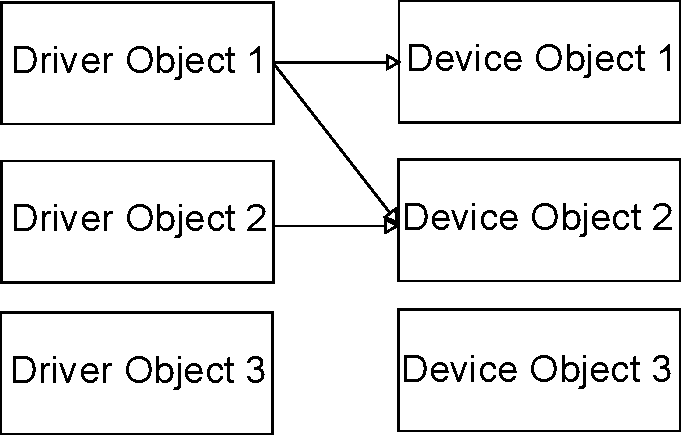
\includegraphics[width=0.6\linewidth]{./graph/drv-to-dev}
\caption{设备对象和驱动对象的对应关系}
\label{fig:drv-to-dev}
\end{figure}

从功能的角度讲,WDM驱动模型被分为三类:
\begin{enumerate}
\item
总线型驱动:驱动某种类型的计算机总线设备,为这种总线上挂载的每个设备提供独立的功能接口。检测和处理总线类型设备的加载和移除事件,负责总线上硬件的驱动程序注册、卸载和仲裁等管理工作。
\item
功能型驱动:驱动某种指定类型的硬件设备,通过和设备间的数据交互实现某一功能,并提供给上层应用程序访问硬件的API接口。如果设备挂载在某种数据总线上,还需要向总线驱动注册总线事件的回调函数。一般由硬件生产厂商提供,在大多数硬件环境下,一个功能型驱动会服务多个硬件设备。
\item
过滤器型驱动:过滤发送给某个设备或是某种类型的硬件总线的操作请求,对捕获到的IO请求进行选择性的处理。过滤器驱动程序对捕获到的请求的处理方式可以是任意的:直接传递给下一个设备对象、处理后再传递或是处理后返回并结束该IO请求。
\end{enumerate}

实践证明,鉴于WDM模型对于驱动程序模块化的组织和规范化的接口要求。使用WDM模型开发硬件驱动程序会使系统内核更加稳定,操作系统可以更高效地操纵硬件。更重要的是,不仅作为驱动程序与操作系统交互的标准接口,WDM还强调驱动程序应该采用模块化的体系架构和设计思想,从而简化调试过程中的错误定位过程。

\subsection{IRP和驱动程序堆栈}
IRP(I/O request package)是Windows内核中描述驱动程序模块之间交互协议的数据描述。上层应用程序通过调用操作系统提供的API函数,进行和设备或文件的交互工作。而API函数的实现中,则需调用IO管理器完成交互请求。IO管理器根据操作的类型将交互信息封装成相应的IRP请求,并发送给对应的设备对象。IRP最终会以调用参数的形式,传递给驱动内部不同类型的分发函数。处理结束后,IO管理器将包含分发函数返回结果的IRP进行解包,返回应用程序的所需信息。

驱动程序堆栈是从应用层API到硬件访问接口的一整套驱动程序。大多数情况下,一个硬件设备能够正常运转依靠的是多个驱动程序的协同工作,这些驱动程序创建的设备对象按消息处理的顺序层次化组合在了一起,构成了设备的驱动程序堆栈。IRP扮演了驱动程序堆栈中层与层之间消息传递的媒介:IRP通过每个设备所唯一对应的驱动程序堆栈,自上而下将用户操作传达至硬件设备;驱动程序将从硬件设备获得的数据存入IRP,自下而上返回给上层应用。

因此,捕获IO操作本质上是捕获驱动程序堆栈中IRP的操作。

\subsection{驱动程序分发函数}
设备对象接收到IRP后,将其作为参数传递给驱动程序的分发函数。驱动程序通过IRP内部保存的分发函数类型码(IRP\_MJ\_XXX)确定用于处理该IRP的分发函数。Windows系统定义了针对不同类型设备的一整套分发函数码。驱动程序要能正常运行,必须实现表\ref{tab:must-handled-major-function}中的所有分发函数。

\begin{table}[H]
\centering
\caption{驱动程序必须提供的分发函数}
\begin{tabular}{|ll|}
\hline IRP\_MJ\_PNP  & 识别、配置PnP设备,分配硬件资源。 \\
       IRP\_MJ\_POWER & 处理电源管理器发出的电源请求。 \\
       IRP\_MJ\_CREATE & 处理用户程序打开设备对象的操作。 \\
       IRP\_MJ\_CLOSE & 处理用户程序关闭设备对象的操作。 \\
       IRP\_MJ\_READ & 处理用户程序对设备对象的读操作。 \\
       IRP\_MJ\_WRITE & 处理用户程序对设备对象的写操作。 \\
       IRP\_MJ\_DEVICE\_CONTROL & 公共IOCTL处理函数。 \\
       IRP\_MJ\_INTERNAL\_DEVICE\_CONTROL & 私有IOCTL处理函数。 \\
       IRP\_MJ\_SYSTEM\_CONTROL & 处理系统发送给驱动程序的管理指令。 \\
\hline
\end{tabular}
\label{tab:must-handled-major-function}
\end{table}

表\ref{tab:option-handled-major-function}中的分发函数则不是必须的,驱动程序可根据实际情况选择性实现。

\begin{table}[H]
\centering
\caption{驱动程序选择性提供的分发函数}
\begin{tabular}{|ll|}
\hline IRP\_MJ\_CLEANUP & 执行用户程序关闭设备对象前的清理工作。 \\
       IRP\_MJ\_QUERY\_INFORMATION & 处理来自用户程序或是内核组件对设备对象的信息请求。 \\
       IRP\_MJ\_SET\_INFORMATION & 处理来自用户程序或是内核组件对设备对象的属性设置。 \\
       IRP\_MJ\_FLUSH\_BUFFERS & 将设备对象Buffer中缓存的数据写回到物理设备。 \\
       IRP\_MJ\_SHUTDOWN & 处理操作系统请求的重启、待机和关机事件。 \\
\hline
\end{tabular}
\label{tab:option-handled-major-function}
\end{table}

分发函数处理IRP的最简单方式是直接传递给驱动程序堆栈中下一层的设备对象,除此之外还可以在进行一定处理后传递或者直接结束来自IRP的IO请求。

\subsection{存储卷过滤器驱动}
设计驱动程序堆栈这一框架,除了能够层次化的管理驱动程序,另一个目的就是使得在功能型的驱动之间加入过滤器驱动程序\cite{filterdrv2004}成为可能。

在任意某个驱动程序堆栈中,可以加入任意多个过滤器驱动程序。一个典型的驱动程序堆栈的组成结构如图\ref{fig:io-stack-filter}所示。过滤器类型驱动程序并非设备运行所必须,因而图中以虚线画出。
\begin{figure}[H]
\centering
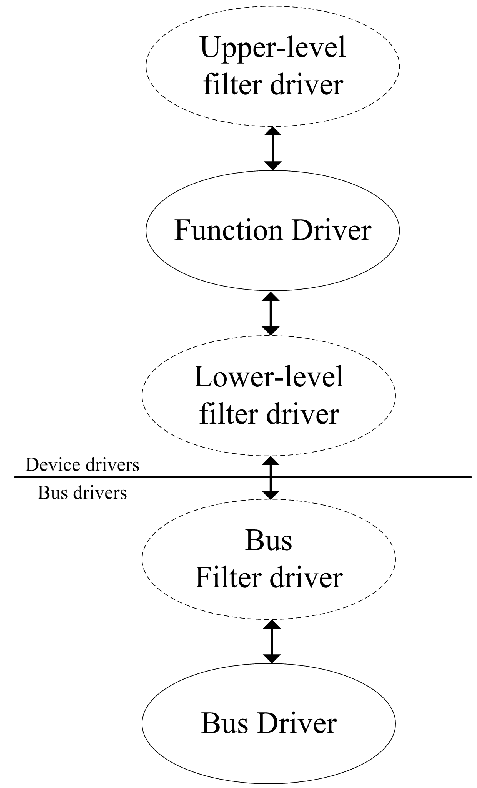
\includegraphics[width=0.4\linewidth]{./graph/io-stack-filter}
\caption{驱动程序堆栈和过滤器驱动程序}
\label{fig:io-stack-filter}
\end{figure}

存在三种类型的过滤器驱动程序:

\begin{enumerate}
\item
总线过滤器驱动:过滤、处理总线事件,将总线的硬件信号转换为驱动程序能够处理的总线事件,管理总线上挂载的设备对象,为总线设备加入新的功能。
\item
底层过滤器驱动:位于功能型驱动程序之下,用于改变设备展现给功能型驱动程序的硬件行为,使功能型驱动程序按照期望的方式运行。
\item
上层过滤器驱动:处于功能型驱动程序之上,过滤应用程序发送给设备的由IO管理器封装为IRP的IO请求。过滤到的IRP多为抽象程度高、硬件相关度低的IO请求。
\end{enumerate}

本论文实现的机械硬盘存储卷的过滤器驱动,是一种存在于机械硬盘所属的驱动程序堆栈中的上层过滤器驱动程序。

\section{缓存页面替换算法}
\label{sec:cache_algorithm}

伴随着应程序访问存储设备,不断会有新的数据加入到缓存空间。当缓存中已经没有空闲的存储空间,而此时又有新的主存数据可以加入时,就需要使用缓存页面替换算法选择性地释放空间,从而容纳新进数据。

常用的缓存页面替换算法按照替换策略可分为基于时间和基于频度的两类,本缓存系统对这两种类型的替换算法都进行了实现。除此之外,本论文还提出了一种新的缓存页面替换算法,该算法综合考虑了缓存块访问时间和访问频度因素。缓存系统运行时,可任意从这三种中选择其中一种使用。

\subsection{基于访问时间的LRU(Least Recently Used)系列替换算法}

LRU替换算法\cite{LRU}通过缓存块最后一次访问距离当前的时长进行决策。当缓存没有空闲空间时,替换出最近最不使用的(距上次访问时间最长的)缓存块。

虽然LRU替换算法根据访问时间进行替换决策,但实现时并不需要为每个缓存块记录访问时间,而是使用链表的方式组织缓存块:根据缓存块在链表中的位置记录缓存块最后一次访问距离当前的时长。

缓存块链表存在冷、热两端。当存在空闲的缓存块时,新缓存块会由热端加入。运行中被访问的缓存块从链表中的任意位置移动到热端。当需要加入新缓存块而缓存链表又已经满时,从链表的冷端移除缓存块,替换数据后加入到链表热端(图\ref{fig:replace-algo-lru})。从热端到冷端,链表中的元素均按照最近一次访问时间的递减顺序排列。

\begin{figure}[H]
\centering
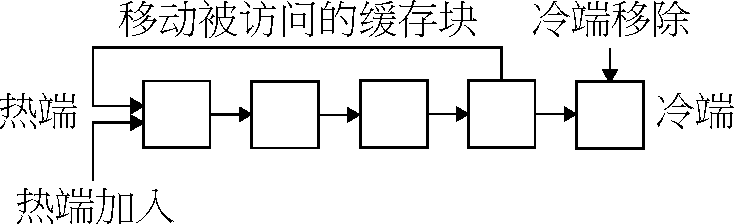
\includegraphics[width=0.6\linewidth]{./graph/replace-algo-lru}
\caption{使用链表的LRU缓存替换算法}
\label{fig:replace-algo-lru}
\end{figure}

LRU替换算法实现简单,能够以很低的性能开销适应变化的数据访问。存在的缺点是,对于考虑数据的长期访问特性没有做出很好的处理。最近使用的缓存块可能并不会被经常访问;经常访问的数据也可能因为暂时不使用而被换出,导致更需要留在缓存中的数据块被替换出去。

\subsection{基于使用频度的LFU(Least Frequently Used)系列替换算法}

LFU替换算法\cite{LFU}利用缓存块的访问频数进行决策。当缓存中不存在空闲的缓存块时,替换出历史访问频度最小的缓存块。

新加入的缓存块初始访问频度为1,随系统运行动态调整访问频度。为了在最短时间找到被替换出的缓存块,实现中使用小顶堆数据结构进行缓存块的组织,堆顶元素总是访问频度最低的元素,随时可以被替换出去。

LFU算法需要为每个缓存块设置一个记录访问频度的区域,以保存访问次数。使用了小顶堆数据结构实现替换策略,实现难度略高于LRU。缺点是需要一定策略对计数器进行清零,否则计数器只增不减会导致某些曾经被频繁访问的缓存块无法及时地被清理出去;新加入缓存块访问频度低,在缓存中停留较短时间后就会被替换出去。

\subsection{综合考虑时间和访问频度的替换算法}

上述两种缓存页面替换算法在选择缓存块时,都存在只考虑最后一次的访问时间或使用频度等某一项因素进行评估的缺陷。为了克服这种缺陷,本论文提出了一种综合考虑访问时间和使用频度的替换算法,该算法实现简单,且测试结果表明命中率优于LRU和LFU替换算法。以下是该算法的缓存块组织方式和处理逻辑:

替换算法使用冷、热两个链表管理缓存块(图\ref{fig:replace-algo-1}),初始状态下两个链表均为空,代表缓存中还没有开始缓存数据。类似于LRU,每个链表都存在冷、热两端,缓存块在链表中的位置代表了缓存块最近一次访问的时间。两个链表的容量上限之和代表了缓存的总容量。
\begin{figure}[H]
\centering
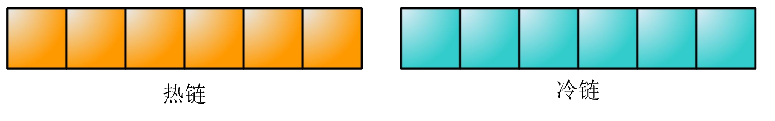
\includegraphics[width=0.6\linewidth]{./graph/replace-algo-1}
\caption{替换算法使用两个链表管理缓存块}
\label{fig:replace-algo-1}
\end{figure}

当冷链表不为满时,新到来的缓存块首先会被加入到冷链表的热端,在运行过程中会统计每个缓存块的访问计数(初始为1)。如果某个缓存块被访问,该缓存块无论在冷链还是热链都会被移动到该链表的热端,并且访问计数增加1。图\ref{fig:replace-algo-2}展示了缓存块以A->B->C->D->E的字母表顺序加入缓存后的组织状态。
\begin{figure}[H]
\centering
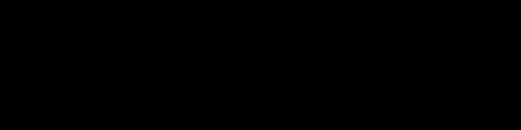
\includegraphics[width=0.6\linewidth]{./graph/replace-algo-2}
\caption{新到来的缓存块加入到冷链表}
\label{fig:replace-algo-2}
\end{figure}

随着缓存系统的运行以及缓存块的不断加入。当冷链表已满,而又要加入新的缓存块时。则需从冷链中移出一部分缓存块以释放空间,新的缓存块仍旧会被加入到冷链的热端。缓存算法会判断被移出缓存块的引用计数,如果其引用计数大于等于2,则清零其引用计数,并加入到热链表的热端;否则该缓存块空间将会被释放。图\ref{fig:replace-algo-3}展示了加入块G移出块A的过程。
\begin{figure}[H]
\centering
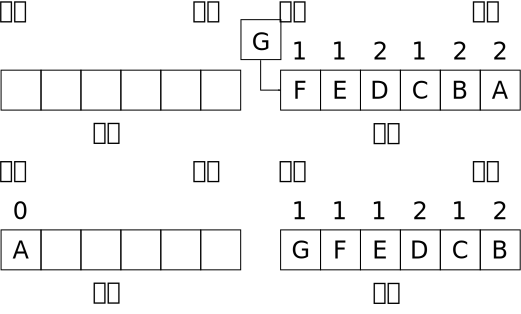
\includegraphics[width=0.6\linewidth]{./graph/replace-algo-3}
\caption{冷链表满时加入缓存块的处理策略}
\label{fig:replace-algo-3}
\end{figure}

新缓存块的持续到来导致冷链表中的缓存块不断被移动到热链表,热链表也会逐渐变满。当热链表中也不存在空闲空间时,加入新缓存块,热链表冷端的缓存块会像图\ref{fig:replace-algo-3}中冷链表的冷端的缓存块一样被换出。从热链中被换出的缓存块的引用计数会被清零,然后加入到冷链表的热端,重复图\ref{fig:replace-algo-3}的过程。整个过程在图\ref{fig:replace-algo-4}中描述。
\begin{figure}[H]
\centering
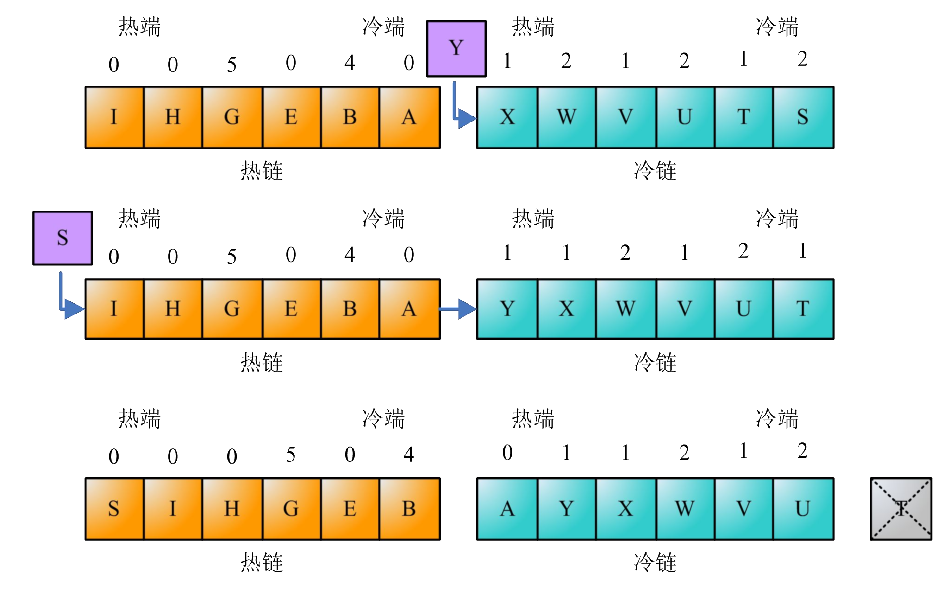
\includegraphics[width=0.7\linewidth]{./graph/replace-algo-4}
\caption{冷热链表均满时加入缓存块的处理策略}
\label{fig:replace-algo-4}
\end{figure}

本替换算法的核心思想是:冷、热链表内部完成LRU替换算法;冷、热链表之间完成LFU替换算法。单独观察冷或热链表,实质就是一个LRU算法管理的链表。缓存块在两个链表之间移动时,考虑到了访问频度的因素,这一点则反映了LFU替换算法的思想。

\section{缓存映射策略}
\label{sec:cache_mapping}

缓存映射策略指的是从主存空间到缓存空间之间的映射关系,缓存映射策略的选择直接决定了缓存系统的实现结构和运行效率。目前,存在三种使用场景最多的缓存块映射策略\cite{cachemap2013}。

\subsubsection{直接相联映射}

主存储器中的每一块空间,都被映射到了缓存中的某块指定的存储空间中。每个缓存块关联了主存中的一个或多个存储空间(图\ref{fig:cache-map-1})。

\begin{figure}[H]
\centering
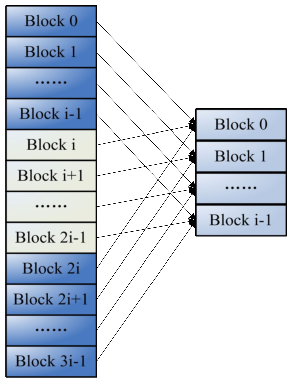
\includegraphics[width=0.4\linewidth]{./graph/cache-map-1}
\caption{直接相联映射}
\label{fig:cache-map-1}
\end{figure}

映射规则:
\begin{itemize}
\item 按相同大小的数据块划分主存与缓存空间。
\item 主存容量和缓存容量是整数倍的关系。将主存空间按缓存容量进行分区,主存每个区域内的块数等同于总的缓存块数。 
\item 主存中某区的一块数据,只能存入缓存中偏移与该块数据距离主存区域开始的距离相同的位置。
\end{itemize}

以主存地址x映射到缓存地址y为例,则x和y满足如下关系。
y = x mod m	(M为缓存的总大小)
直接映射方式的优点是实现简单,可以使用主存地址直接计算出对应的缓存地址,不存在查找过程。缺点是缓存中的每个存储块通常对应主存中多个固定的存储块,运行中如果存在多个块同时被访问会产生缓存替换策略被频繁调用的情况。因此,直接映射适合缓存容量为主存的30\%以上时采用,一般应用于超大型系统。

\subsubsection{全相联映射}

与直接相联的固定映射方式相反,全相联映射缓存中的每一块都可映射给将主存的任一块数据(图\ref{fig:cache-map-2})。

\begin{figure}[H]
\centering
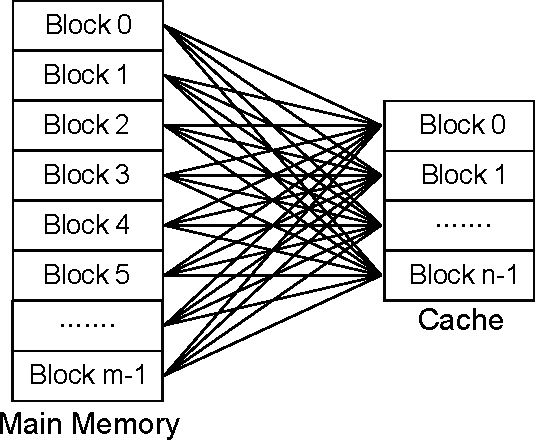
\includegraphics[width=0.4\linewidth]{./graph/cache-map-2}
\caption{全相联映射}
\label{fig:cache-map-2}
\end{figure}

映射规则:
\begin{itemize}
\item 按相同大小的数据块划分主存与缓存空间。
\item 缓存的每一块都可映射给主存的任意一块数据。缓存块总数是N,主存块总数是M时,存在多达N×M种的映射关系。
\end{itemize}

全相联映射的优点是主存和缓存的容量没有限制,只需按照相同大小的数据块进行组织。缺点是在不使用额外的索引数据结构的情况下,当查询主存中的某个数据块是否被缓存时,需要遍历所有缓存块进行查找。为提高查找效率,必须要使用辅助的查找数据结构建立索引,使用额外的空间存储索引也必不可少。

\subsubsection{组相联映射}

主储存器的每一组都与缓存中的某一组相对应,组内的每个块与缓存组内的任意一个存储块相映射(图\ref{fig:cache-map-3})。

映射规则:
\begin{itemize}
\item 按相同大小的数据块划分主存与缓存空间。
\item 主存与缓存以相同数量的数据块划分成组。
\item 主存内组的数目是缓存内总组数目的整数倍。
\end{itemize}

\begin{figure}[H]
\centering
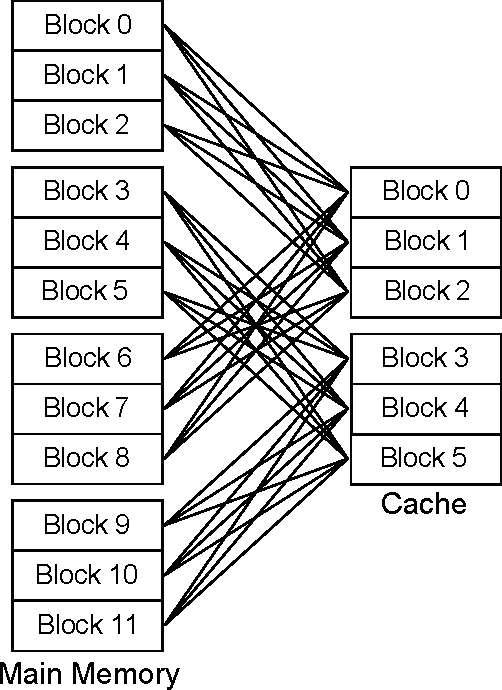
\includegraphics[width=0.4\linewidth]{./graph/cache-map-3}
\caption{组相联映射}
\label{fig:cache-map-3}
\end{figure}

当检测缓存是否命中时,先使用主存地址求出其唯一对应的缓存组,既主存组内的某一块只能存入同一组号的缓存组内。相关联的两组内各存储块之间的映射关系任意,这一方面类似于全相联映射。组与组之间的映射关系固定,这一方面类似直接相联映射。

一般会从三个角度比较这几种映射策略。
\subsubsection{索引速度}
直接映射可以直接计算出缓存地址,不需要查找,速度最快;组相联方式则需要查找对应的缓存组,速度次之;全相联映射的查询最为复杂。
\subsubsection{缓存利用率}
全相联方式主存和缓存块之间的映射关系任意,缓存利用率最高;组相联方式组内映射任意,但是组间相互独立,利用率次之;直接映射缓存中的每个缓存块与主存中的一个或多个存储块相关联,利用率最低。
\subsubsection{实现难度}
直接映射方式计算复杂度最低,适合硬件实现;组相联方式和全相联映射方式的实现难度取决于使用的索引数据结构。组相联方式可以在组内块数量较少时使用遍历的方法,这种实现也相对简单。

\section{缓存索引数据结构}
\label{sec:cache_indexing}

缓存系统使用缓存索引数据结构查询某个主存块是否被缓存、定位缓存块在缓存中的位置。缓存系统所选用的映射策略,决定了对应的缓存索引数据结构。

使用直接相联映射结构,主存储器中的每个数据块,根据地址的映射关系,对应了缓存中唯一的一个缓存块。因此,使用直接相联映射策略时,不需要额外的缓存索引结构支持缓存块的查找,使用主存地址直接计算就可以得知该主存块是否被缓存。

使用全相联映射结构,主存储器中的每个数据块和缓存中的每个数据块的存储地址之间没有任何的关系,主存储器的一个数据块可以映射到缓存中的任意某个缓存块的位置。使用全相联映射结构,进行缓存块的查找时,为了避免遍历查找带来的延迟,就不得不需要某种额外的索引数据结构定位主存储块映射的缓存块地址。

如果选用组相联方式,则是折中了直接相联和全相联两种映射结构。组相联映射将主存储器和缓存空间分成个数相同的存储块组,思想类似于直接映射。主存和缓存相联的两组内的主存块和缓存块之间的任意映射关系又等同于全相联映射的思想。在设计缓存系统的过程中需要决定分组的大小:当每个分组内的缓存块数量较少时,查找时可使用实现简单的遍历方法,不需要额外的索引数据结构;当分组内缓存块数量较多时,则和全相联映射一样,需要额外的索引数据结构避免查找带来的长的延迟。

从组织方式上分,索引数据结构分为单级结构、多级结构和树形结构三种类型。

\subsection{单级有序索引}
单级有序索引,顾名思义,就是只需要查询一级,便可以完成从主存储器地址到缓存地址空间的转换,索引结构是线性的。通常使用数组或是链表这类简单数据结构即可满足需求。

\subsubsection{数组方式}
使用静态数组为缓存中的每一个缓存块建立一个索引标签,标签记录了缓存块映射所到的主存储块,未映射时标记为空。索引需要遍历数组元素进行查找。优点是实现简单。缺点是需要在初始化阶段给所有的缓存块建立索引标签,如果缓存空间大,则需要的空间太多,索引速度慢。

\subsubsection{链表方式}
使用双向链表为每一个已经使用的缓存块建立一个索引标签,链表中的所有标签按照缓存地址的大小顺序排列。通过加入、删除和更新链表元素的方式实现缓存映射的更新。相对数组,链表可以在运行时动态分配所需空间。但索引时仍需要遍历所有元素。

\subsection{多级有序索引}

多级索引,是对单级索引空间从横向或者纵向进行多级划分,解决超大容量缓存空间的检索效率问题。由于几个不同种类的单级索引组合在一起,就可以构成一种新的多级索引方法。因此,多级索引的种类繁多。

\subsection{B+树索引}
B+树\cite{bplustree2012}是一种树形索引数据结构,通常用于数据库系统设计和文件系统在磁盘上索引的实现中。B+树的插入与删除操作的 时间复杂度非常稳定。而且因其自底向上的元素插入方式,与红黑树恰恰相反。

\subsubsection{B+树的节点结构}

B+树中的节点内部都会保存一组有序的索引和一组有序的节点指针。如果B+树的阶(order)是m,那么除了当只有一个叶子节点时,每个节点都最少包含m/2个,最多包含m-1个索引。内部节点的节点指针的数目总是比索引的数目多一个,内部节点的节点指针总是指向下一层的内部节点。所有叶子节点处于同一层的高度,其内部的索引数目和有效元素指针(节点指针)的数目相同,节点指针指向被索引的数据。图\ref{fig:bplus-tree}展示了一棵阶为4的B+树。

通常称B+树内部节点保存的每个索引值为分离值。例如,某个内部节点存在两分离值(元素)$a_1$和$a_2$,则其必须存在三个子指针指向其子树:左子树的所有节点的元素值均小于$a_1$,中间子树所有节点的元素值处于$[a_1,a_2)$区间,右子树的所有节点的元素值均大于等于$a_2$。

\subsubsection{B+树的查找算法}

B+树的查找算法类似于排序二叉树:从根节点开始,自顶向下遍历树的节点,根据要查找数据的索引值决定选择分离值哪一边的节点指针。使用子指针进入下一层内部节点,直到进入某个叶子节点。遍历叶子节点的所有元素,查找索引值,如果存在相同元素则找到,否则B+树中不存在查询索引。

\subsubsection{B+树的插入算法}

当节点内元素的树木不属于B+树节点结构的可接受的范围时,这个B+树节点处于违规状态。节点内节点指针的最小数量必须大于m/2。B+树的插入过程要处理节点因包含过多元素而违规的情况,插入过程为:
\begin{enumerate}
\item 根据数据索引值,查找适合的元素插入叶子节点。
\item 将元素插入到叶子节点内部的合适位置上。
\item 此时的叶子节点如果未因包含过多元素而违规,处理结束。
\item 如果此时的叶子节点包含的元素过多,则分裂为两个叶子节点,这两个节点必将拥有最小数目元素。分裂操作会导致上一内部层节点元素指针数目增加,因此需要递归向上处理到根节点。如果根节点也因包含过多元素而被分裂,则创建新的根节点,树的高度也因此而增加。
\end{enumerate}

\subsubsection{B+树的删除算法}

B+树的删除过程要处理节点违规的情况,删除过程为:

\begin{enumerate}
\item 根据索引值,查找到包含被删除元素的叶子。
\item 删除叶子节点内的待删除元素。
\item 如果此时叶子节点没有因元素过少而违规,处理结束。
\item 此时节点可能处于以下两种违规的状态之一,递归向上处理违规的叶子节点,直到不存在违规节点:
\begin{enumerate}
\item 节点的左、右兄弟节点,在不变为违规节点的前提下,可以把一或多个子节点移动到处于违规状态的节点,使其变为合法的节点。在移动子节点内元素后,必然要更新相应节点的分离值,并向上递归处理。
\item 节点的左、右兄弟节点内的元素个数均处于合法个数的下界。这种情况下,将当前节点和左或右兄弟节点合并,再平均分裂为两个节点。更新相应节点的分离值,持续这一过程直到当前节点合法或者合并到达根节点。
\end{enumerate}
\end{enumerate}

\begin{figure}[H]
\centering
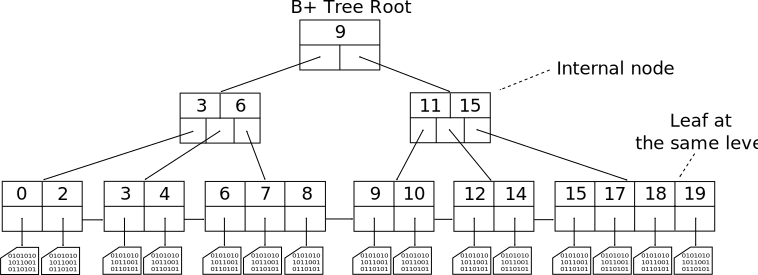
\includegraphics[width=1\linewidth]{./graph/bplus-tree}
\caption{B+树结构}
\label{fig:bplus-tree}
\end{figure}

\section{回写策略}
\label{sec:wb_strategy}

对于应用程序的读请求,主存中的数据不会被改变,因此不存在数据一致性的问题。然而对于应用程序的写请求,需要决定是直接将写请求应用到主存储上还是延迟后再进行写更新,这种延迟写回的策略被称之为回写策略\cite{writeback2014}。

本节将会介绍工程实现中使用最为广泛的三种回写策略:写穿法、写回法和写一次法的原理和实现方式。本论文实现的缓存系统实现了写穿法、写回法两种回写策略,运行时只能选取其中一种策略运行。

\subsection{写穿法(Write Through)}
\begin{figure}[H]
\centering
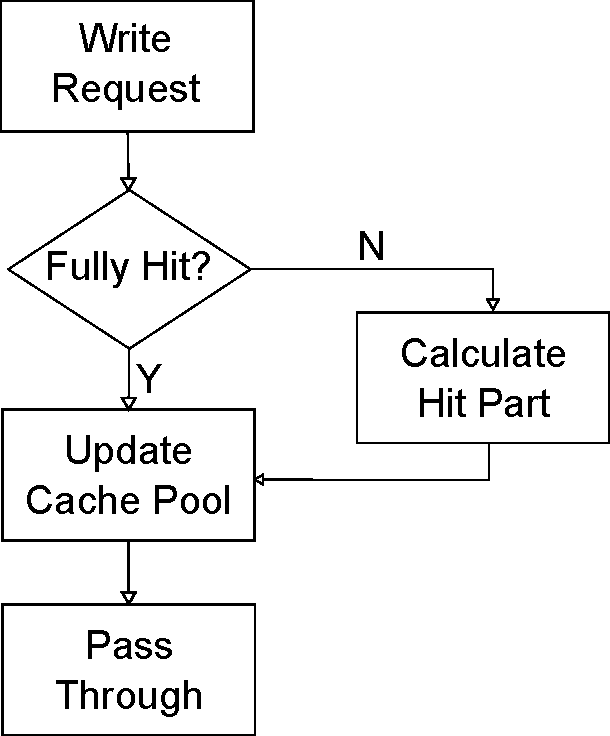
\includegraphics[width=0.4\linewidth]{./graph/write-through}
\caption{写穿法处理策略}
\label{fig:write-through}
\end{figure}

写穿法\cite{writethrough2010}对于接收到的写请求,同时应用于机械硬盘和固态硬盘缓存。由于机械硬盘和固态硬盘缓存数据是同时写入的,因此无需考虑数据一致性问题,也无需为每个缓存块设置标志位记录此缓存块是否被修改过(图\ref{fig:write-through})。

写穿法这种回写策略的缺点是,运行这种回写策略的缓存系统不但无法提升应用程序的写操作的IO性能,相反的,还会造成写性能一定程度的降低。这是因为,如果没有缓存系统,应用程序的写操作直接应用到机械硬盘上即可;存在缓存系统,除了应用到机械硬盘,还要使用写请求的数据更新固态硬盘缓存中命中部分的数据,总的处理时间相对没有缓存反而更长。

\subsection{写回法(Write Back)}
\begin{figure}[H]
\centering
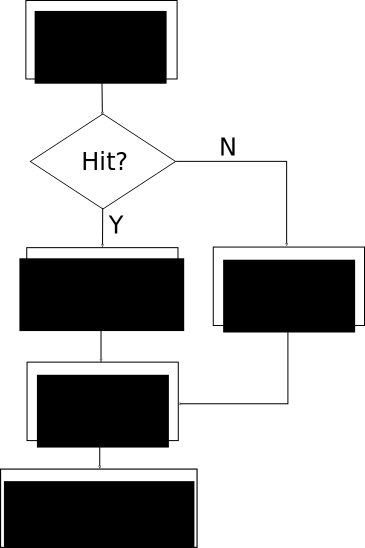
\includegraphics[width=0.4\linewidth]{./graph/write-back}
\caption{写回法处理策略}
\label{fig:write-back}
\end{figure}

写回法\cite{writeback2008}对于接收到的写请求,只将写操作应用于固态硬盘缓存,更新后立即完成写操作请求。写回法需要为每个缓存块设置一个修改位标志,更新后将修改位标志置位,并将缓存块指针加入到回写队列(图\ref{fig:write-back-queue}),回写队列在延迟一定时间后同步机械硬盘数据,同步后清除修改位标志。缓存页面替换算法运行时,不能选择替换修改位标志被置位的数据块。

\begin{figure}[H]
\centering
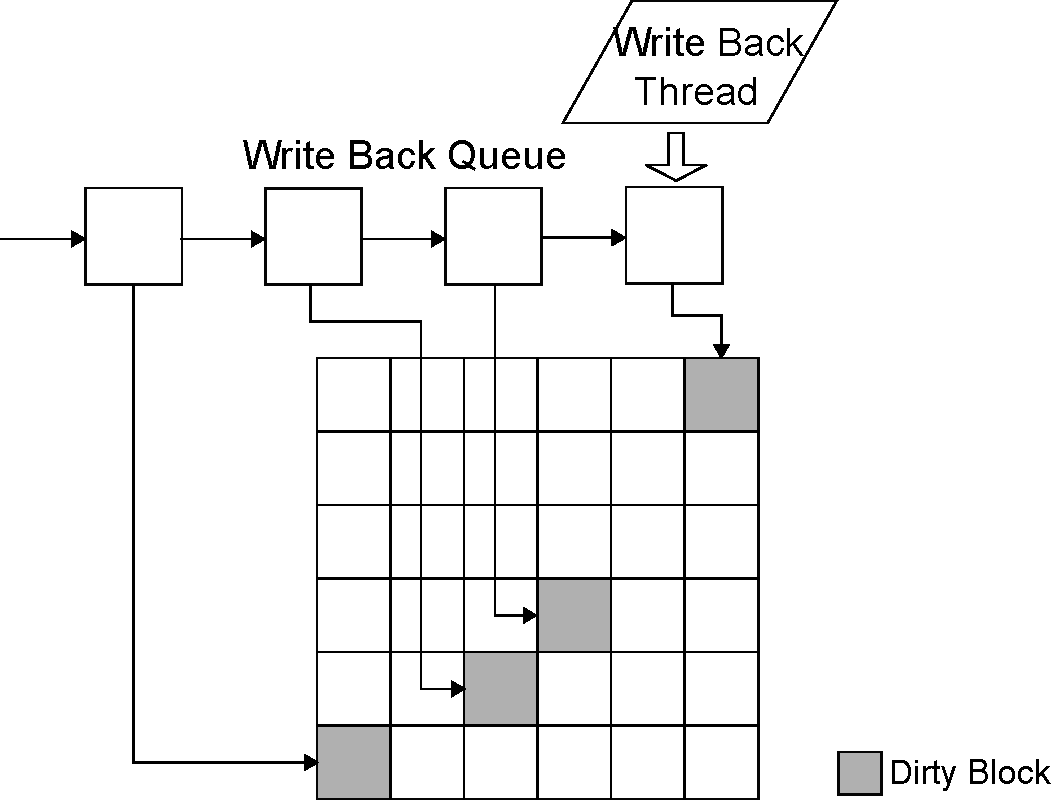
\includegraphics[width=0.6\linewidth]{./graph/write-back-queue}
\caption{指向脏数据块的回写队列}
\label{fig:write-back-queue}
\end{figure}

回写队列的大小是固定的。随着脏数据块的加入,当回写队列满时,会触发回写线程进行写回操作。回写线程将队列中的所有脏缓存块刷回机械硬盘。同样的,当线程接收到回写所有或线程终止信号时,也会进行刷写所有脏缓存块回机械硬盘的操作(图\ref{fig:write-back-thread})。

\begin{figure}[H]
\centering
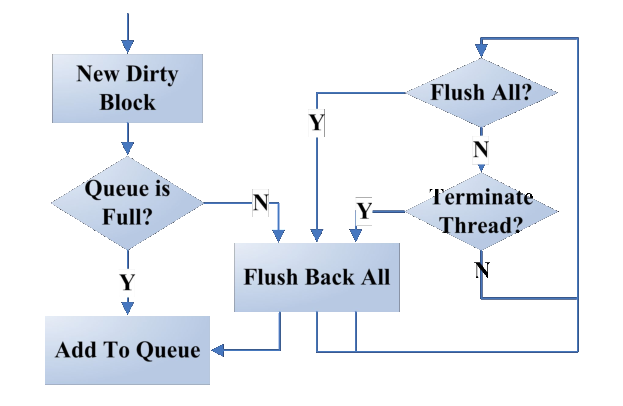
\includegraphics[width=0.6\linewidth]{./graph/write-back-thread}
\caption{回写线程的回写逻辑}
\label{fig:write-back-thread}
\end{figure}

\subsection{写一次法(Write Once)}
写一次法是一种融合了写穿和写回两种方法的回写策略。它的特点是,如果对某个缓存块的写请求命中,只在第一次写更新缓存块时使用写穿策略更新机械硬盘的数据,之后的每次写操作都和写回法一样,只修改缓存内的数据,机械硬盘数据会被延迟写回更新。

实现写一次法,需要为每个缓存块记录该缓存块曾被改写过的次数。

%% ----------------------------------------------------------------------
%%% END OF FILE
%% ----------------------------------------------------------------------
